\documentclass{aes2e}

% Metadata Information
\jyear{2016}
\jmonth{January}
\jvol{1}
\jnum{1}

\usepackage{color,url}
\newcommand{\gregoire}[1]{\textcolor{red}{Gregoire : #1}}
\newcommand{\mathias}[1]{\textcolor{green}{Mathias : #1}}
\newcommand{\ml}[2][]{\textcolor{blue}{#1 #2}}

%\renewcommand{\baselinestretch}{1.5}

\begin{document}
%
% --- Author Metadata here ---
%\CopyrightYear{2007} % Allows default copyright year (20XX) to be over-ridden - IF NEED BE.
%\crdata{0-12345-67-8/90/01}  % Allows default copyright data (0-89791-88-6/97/05) to be over-ridden - IF NEED BE.
% --- End of Author Metadata ---

\title{Semantic browsing of sound databases \\ without keywords}
%\subtitle{[Extended Abstract]
%\titlenote{A full version of this paper is available as
%\textit{Author's Guide to Preparing ACM SIG Proceedings Using
%\LaTeX$2_\epsilon$\ and BibTeX} at
%\texttt{www.acm.org/eaddress.htm}}}
%
% You need the command \numberofauthors to handle the 'placement
% and alignment' of the authors beneath the title.
%
% For aesthetic reasons, we recommend 'three authors at a time'
% i.e. three 'name/affiliation blocks' be placed beneath the title.
%
% NOTE: You are NOT restricted in how many 'rows' of
% "name/affiliations" may appear. We just ask that you restrict
% the number of 'columns' to three.
%
% Because of the available 'opening page real-estate'
% we ask you to refrain from putting more than six authors
% (two rows with three columns) beneath the article title.
% More than six makes the first-page appear very cluttered indeed.
%
% Use the \alignauthor commands to handle the names
% and affiliations for an 'aesthetic maximum' of six authors.
% Add names, affiliations, addresses for
% the seventh etc. author(s) as the argument for the
% \additionalauthors command.
% These 'additional authors' will be output/set for you
% without further effort on your part as the last section in
% the body of your article BEFORE References or any Appendices.

% of EIGHT authors. SIX appear on the 'first-page' (for formatting
% reasons) and the remaining two appear in the \additionalauthors section.
%

%Author Info.
\authorgroup{
\author{Gr\'egoire Lafay$^1$}, \author{Nicolas Misdarris$^2$},
\author{Mathieu Lagrange$^1$}, \author{Mathias Rossignol$^2$}
\email{(gregoire.lafay@irccyn.ec-nantes.fr)}
\affil{IRCCyN, Ecole Centrale de Nantes $^1$ \quad\quad\quad\quad IRCAM, STMS, UPMC $^2$}
}


%\author{
%\alignauthor
% Gregoire Lafay\\
%       \affaddr{IRCCyN, Ecole Centrale de Nantes}\\
%       \affaddr{1 rue de la Noe}\\
%       \affaddr{Nantes, France} 
%       %\email{gregoire.lafay@irccyn.ec-nantes.fr} 
%\alignauthor 
% Nicolas Misdarris\\
%       \affaddr{IRCAM}\\
%       \affaddr{1 Place Igor\-Stravinsky}\\
%       \affaddr{Paris, France} \\
%       \email{}
%\and
%\alignauthor 
%Mathieu Lagrange\\
%       \affaddr{IRCCyN, Ecole Centrale de Nantes}\\
%       \affaddr{1 rue de la Noe}\\
%       \affaddr{Nantes, France} \\
%\alignauthor 
% Mathias Rossignol\\
%       \affaddr{IRCAM}\\
%       \affaddr{1 Place Igor\-Stravinsky}\\
%       \affaddr{Paris, France} \\
%       \email{}
%}       


% There's nothing stopping you putting the seventh, eighth, etc.
% author on the opening page (as the 'third row') but we ask,
% for aesthetic reasons that you place these 'additional authors'
% in the \additional authors block, viz.
%\additionalauthors{Additional authors: John Smith (The Th{\o}rv{\"a}ld Group,
%email: {\texttt{jsmith@affiliation.org}}) and Julius P.~Kumquat
%(The Kumquat Consortium, email: {\texttt{jpkumquat@consortium.net}}).}
\date{26 December 2014 }
% Just remember to make sure that the TOTAL number of authors
% is the number that will appear on the first page PLUS the
% number that will appear in the \additionalauthors section.

\maketitle

\begin{abstract}
~In this paper, we study the relevance of a semantic organization of sounds for easing the browsing of a sound database. For such task, the semantic organization is traditionally hold thanks to a keyword selection process. However, various issues of written language like word polysemy, ambiguities translation issues may bias the browsing process.

We consider here two display of sounds that are organized by considering underlying semantic information that draws a hierarchy. For the sake of comparison, we also consider a display whose organization of sound in the plane is based on acoustic cues. Those three displays are evaluated in terms of search speed in a crowd sourcing experiment. Results 
\end{abstract}

%% A category with the (minimum) three required fields
%\category{H.2.8}{Database Management}{Database Applications}[Data mining]
%%%A category including the fourth, optional field follows...
%\category{D.2.8}{Software Engineering}{Metrics}[complexity measures, performance measures]

%\terms{Design, Experimentation, Human Factors}

\keywords{Audio content management and display, Semantic sound data mining}

\section{Introduction}

With the growing capability of recording and storage, the problem of indexing large databases of audio has recently been the object of much attention \cite{Wold1996}. Most of that effort is dedicated to the automatic inference of indexing metadata from the actual audio recording \cite{Zhang1999, tzanetakis2002musical}; in contrast, the ability to browse such databases in an effective manner has been less considered.


Most media assets management are based on keyword-driven queries. The user enters a word which characterizes the desired item, and the interface presents him with items related to this word. The effectiveness of this principle is primarily based on the typological structure and nomenclature of the database. However, for databases and more specifically for databases of sounds, issues arise:

\begin{enumerate}
\item Sounds, as many others things, can be described in many ways. Sound may be designated by their
sources (a car door), as well as by the action of those sources (the slamming of a car door) or their environments (slamming a car door in a garage) \cite{houix2012lexical, niessen2010categories, brown2011towards}. Designing an effective keyword-based search system requires an accurate description of each sound, which has to be adaptable to the sound representation of each user.
\item Pre-defined verbal descriptions of the sounds made available to the users may potentially bias their browsing and final selection.
\item Localization of the query interface is made difficult as the translation of some words referring to qualitative aspects of the sound such as its ambiance is notoriously ambiguous and subject to cultural specificities.
\item Unless considerable time and resources are invested into developing a multilingual interface, any system based on verbal descriptions can only be used with reduced performance by non-native speakers of the chosen language.
\end{enumerate}

To circumvent those issues, not relying on keywords is desirable. That said, semantics, which is traditionally conveyed through written text, may be important for easing browsing.  

To study this issue, we consider in this paper several means of displaying sounds without relying on any textual representation. One, considered as a reference baseline, do not rely on any semantic information as the sounds are organized according to their acoustical properties, \textit{i.e.} time averaged spectral features. The second one 

Their effectiveness is studied with a search-based task whose aim is find a target sound by browsing the database using the display under evaluation.

The paper is organized as follows: in Section \ref{previous} previous work on the topic of sound database browsing is reviewed. Then, the corpus used in this study is described in Section \ref{dataset}. the three displays under evaluation are next described in Section \ref{display}. The crowd sourcing test used to compare those displays is presented in Section \ref{test}. the outcomes of this experiment are discussed in Section \ref{results}.  

\section{Previous work} \label{previous}

Most of the research effort in Sound Design and Music Information Retrieval (MIR) communities is focused on acoustical based indexing and browsing \cite{tzanetakis2003musescape, streich2008music}. Typically, the items (sound effects or pieces of music) are modeled by processing the digital audio waveform using some signal processing pipeline in order to get a compact description for each  items
\cite{coleman2007mused}. Then, statistical projections or embedding techniques, like Principal components analysis (PCA),  Multi Dimensional Scaling (MDS) \cite{schwarz2009sound,Cano2002}, Self Organizing Maps (SOM) \cite{pampalk2004exploring} and the like are used to project the items in a two or three dimensional space while preserving as much as possible distances among items. One of the advantage of such an approach is its ability to scale to very large databases \cite{schwarz2009scalability} as it does not need any kind of manual annotations and allows to search by similarity efficiently according to acoustical properties.

Though, such acoustical models are inherently subject to observation noise and biases. Selecting the most relevant features to achieve the correct projection of the data may only be performed by an expert user. If done \textit{a priori} by an expert or by some above cited dimensionality reduction technique, the induced bias can strongly limit the user in its ability to . In that respect, semantic tags, if available for the data at hand have the advantage of implicitly structuring the similarity space, thus eventually easing the browsing process even if the actual tags are not -- as in this study -- exposed to the user.

\section{Dataset} \label{dataset}


\begin{figure}[t]
\begin{center}
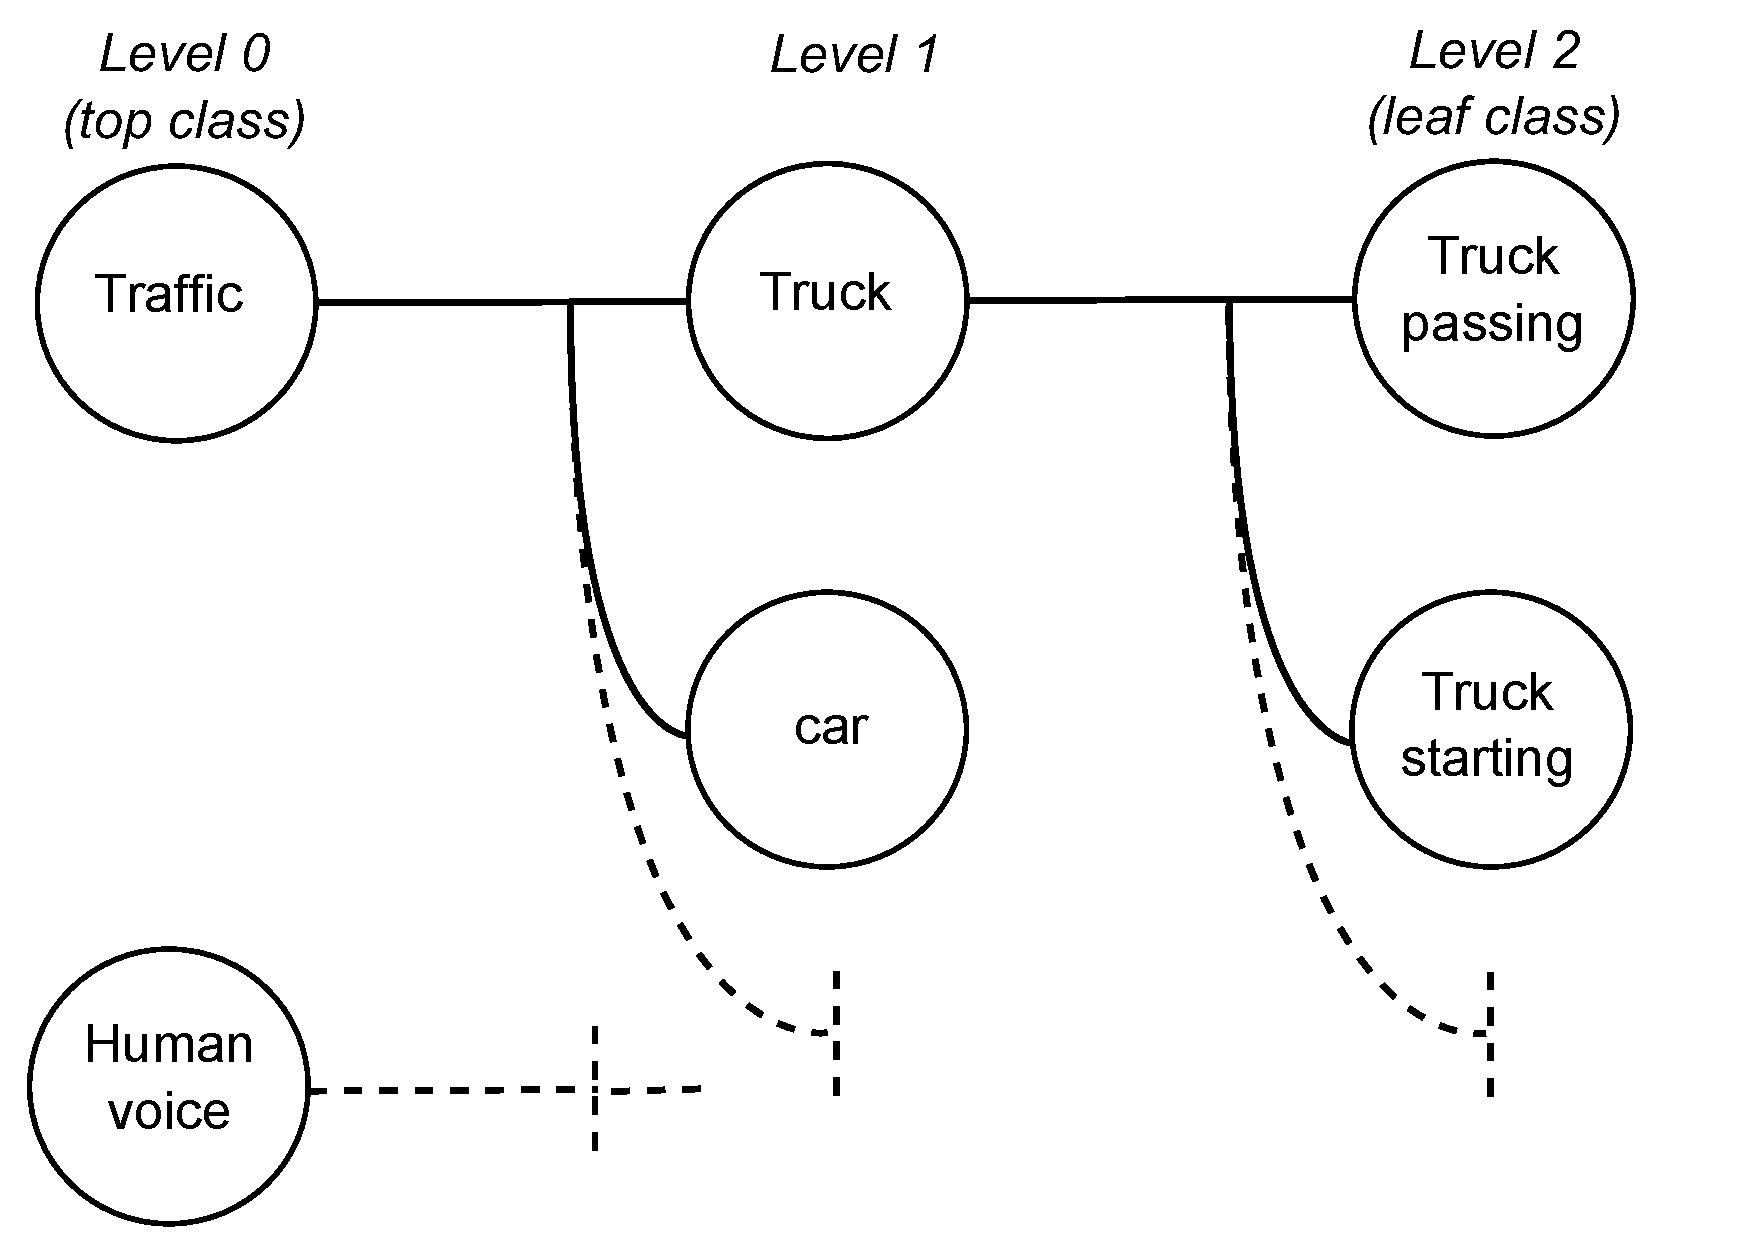
\includegraphics[scale=0.24]{gfx/dataset.pdf} 
\end{center}
\caption{\label{figdataset} Semantic hierarchical structure of the dataset of urban environmental sounds}
\end{figure}

\begin{figure}[t]
\begin{center}
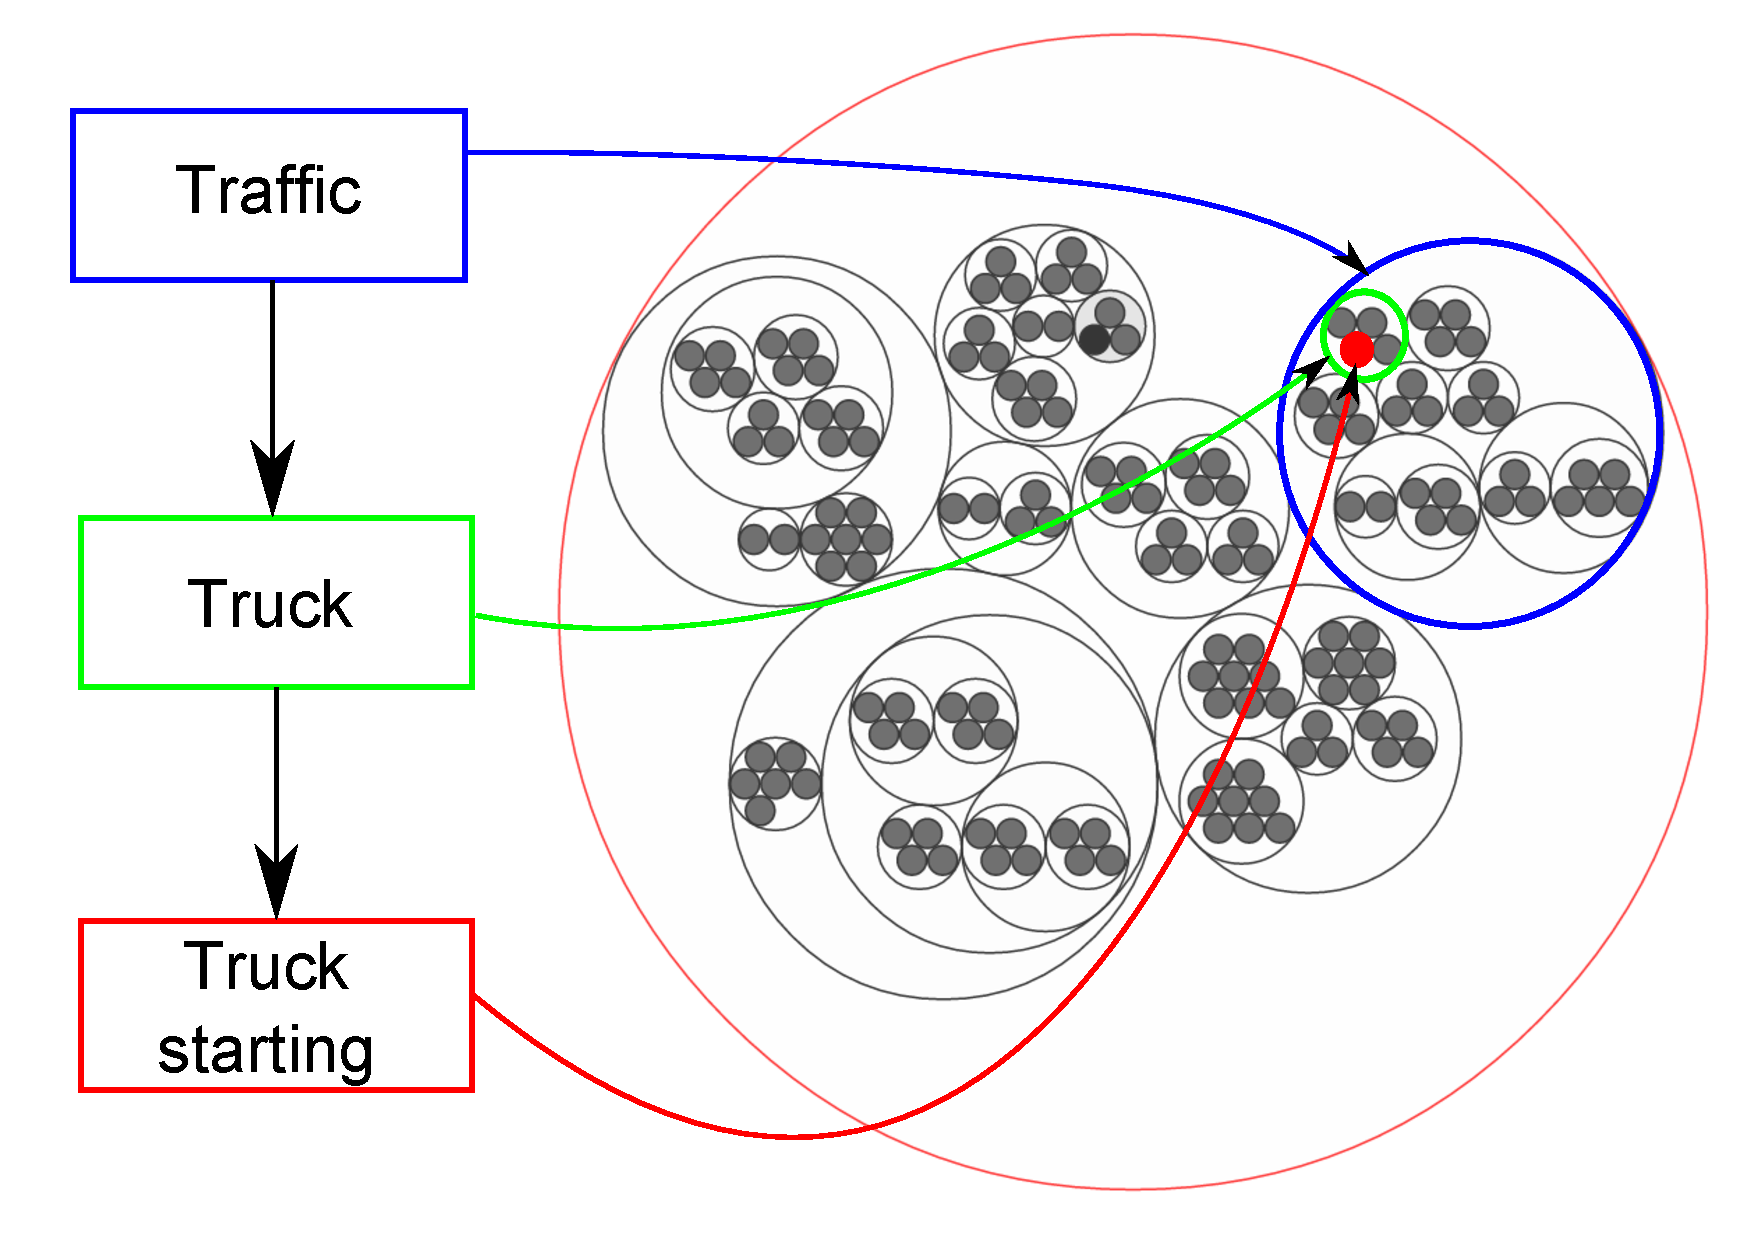
\includegraphics[scale=0.24]{gfx/SSF.pdf} 
\end{center}
\caption{\label{figSSF} Spatial configuration of the Progressive Semantic Display (PSD) based on the semantic hierarchical structure of the dataset}
\end{figure}


The dataset considered in this study is composed of 149 urban environmental sound events. It has a semantic organization that is as follows: a sound is characterized by a tag describing the physical source of the sound (\textit{man-yelling}, \textit{car-passing}). Sounds are then hierarchically grouped into classes according to their tags (\textit{car} $>$ \textit{car-passing}; car $>$ \textit{car-starting}). Those classes are in turn  packed into classes until high level classes describing broader concepts are reached (\textit{traffic} $>$ \textit{car} $>$ \textit{car-passing}). The sound dataset is thus organized into a hierarchical structure of semantic classes as described in Figure~\ref{figdataset}. Strictly speaking, the sound samples of the dataset are the leaf semantic levels. All the other classes are represented by a \textit{prototype sound} that best characterizes the sounds belonging to the class. 

In order for the semantic hierarchical structure to be perceptually valid, the \textit{tags} describing the classes  are chosen from sound categories presented in studies addressing environmental auditory scenes perception \cite{niessen2010categories, brown2011towards, dubois2006cognitive}. In cognitive psychology, sound categories may be regarded as intermediaries between collective sound representations and individual sensory experiences \cite{dubois2006cognitive}. It is our belief that using such category names to build the hierarchical structure makes the latter perceptually motivated, and can thus help the users for efficiently browsing the dataset.


%We choose to represent each sound leaf class of our sound data set with a circle. Circles are dispatched in a 2D space and packed together according to the hierarchical structure of the sound set (see figure \ref{SSF}). The class is identified by listening to an acoustic prototype chosen by the authors for its representativeness. Clicking on a circle fires this audio prototype.

\section{Displays} \label{display}

\begin{figure}[t]
\begin{center}
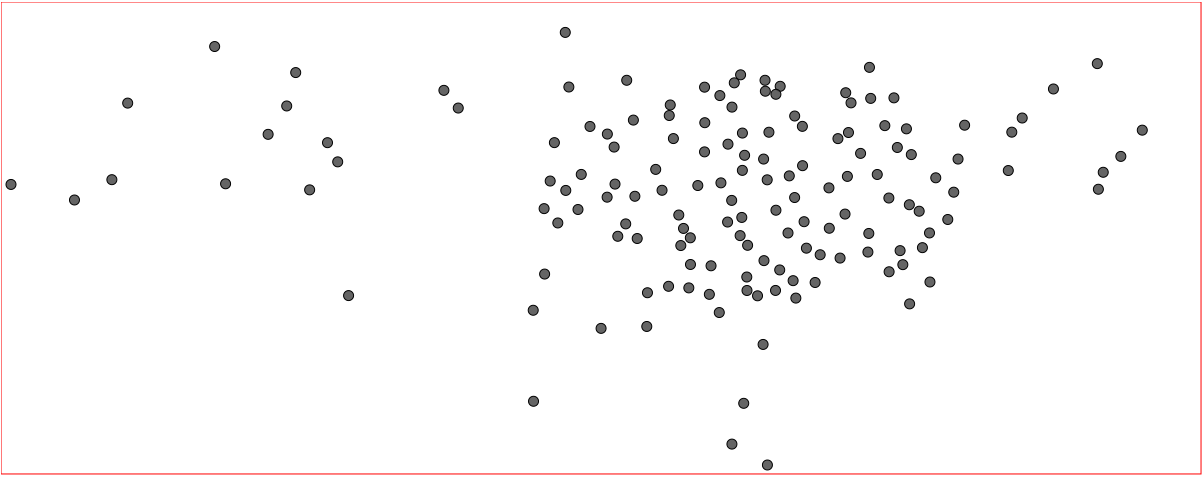
\includegraphics[scale=0.18]{gfx/xp3.png} 
\end{center}
\caption{\label{figXP3} Acoustical Display (AD)}
\end{figure}

\begin{figure}[t!]
\begin{center}
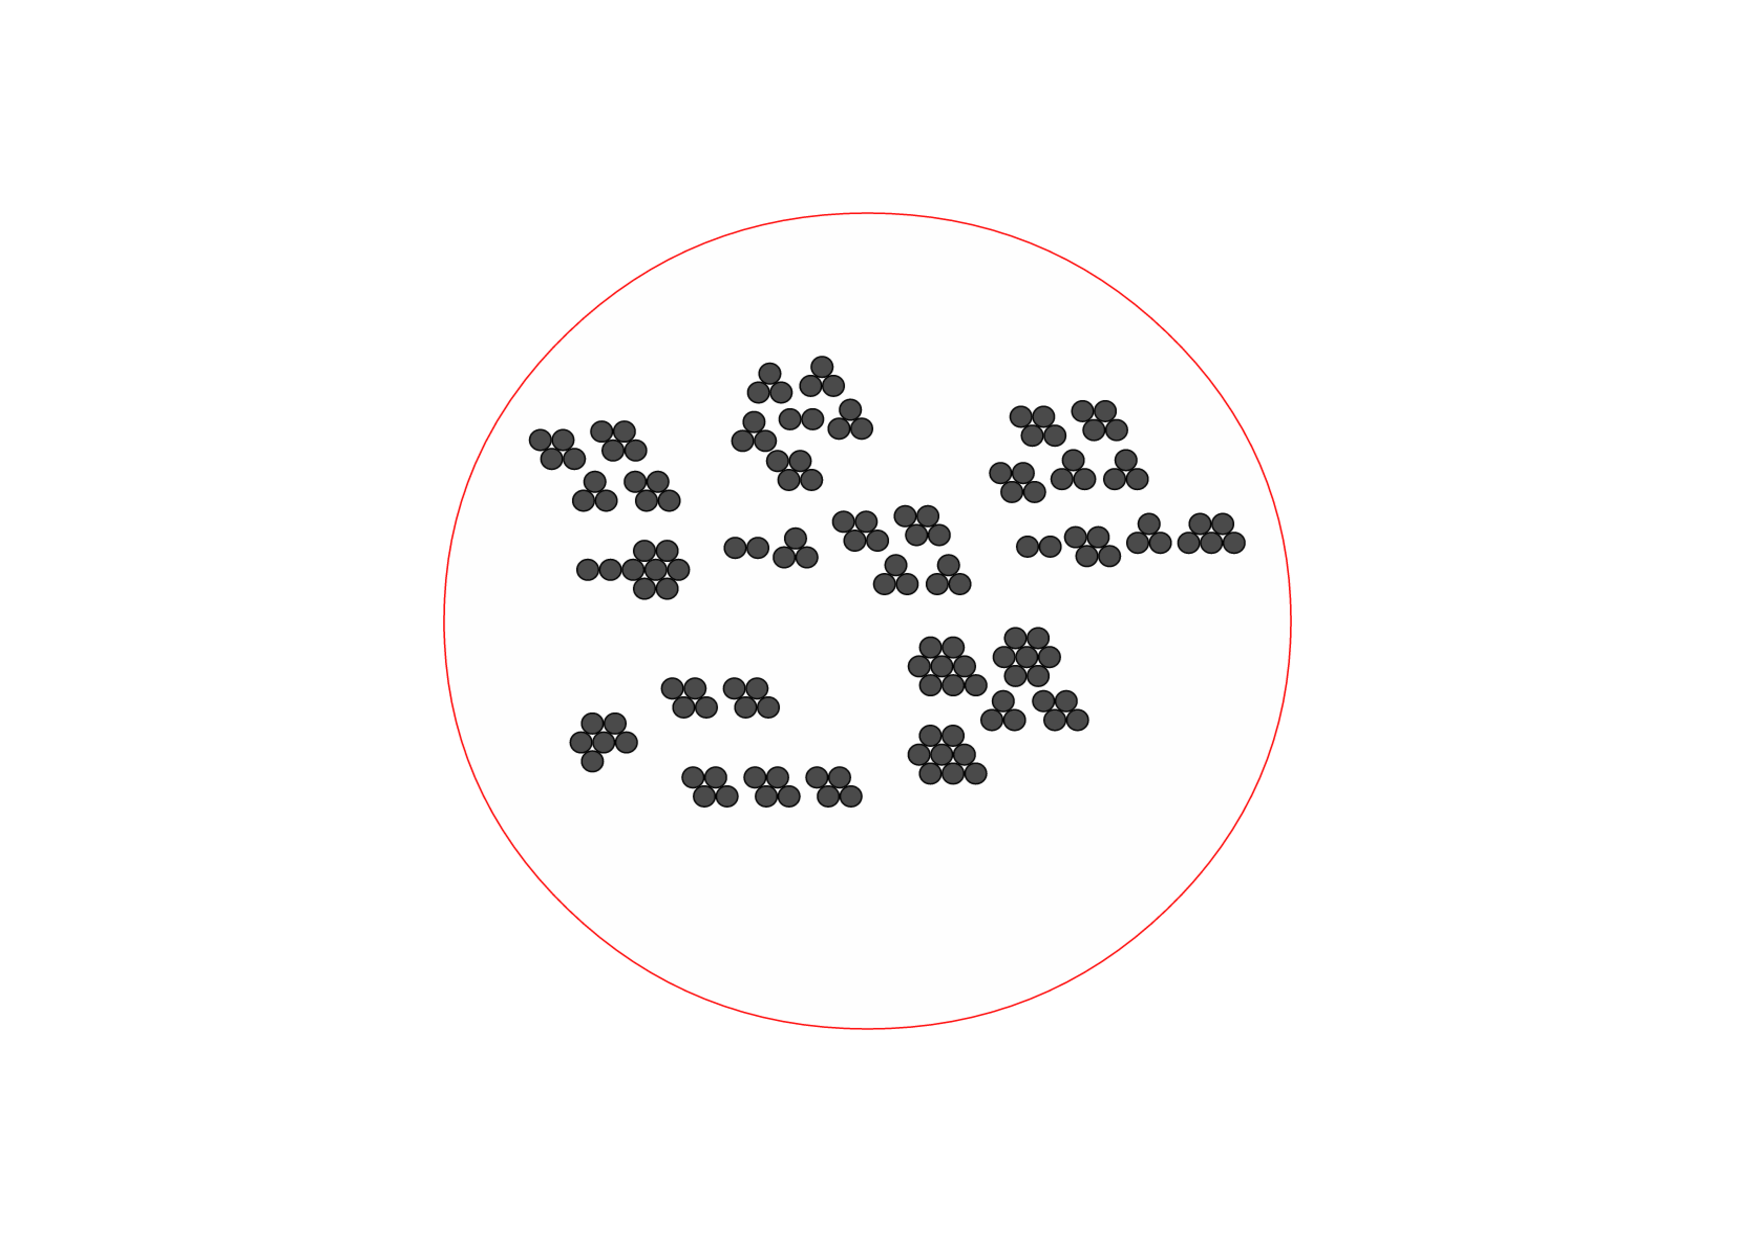
\includegraphics[scale=0.30]{gfx/XP2clean.pdf} 
\end{center}
\caption{\label{figXP2} Full Semantic Display (FSD): implicit hierarchical organization of semantic classes }
\end{figure}

\begin{figure*}[t]
\begin{center}
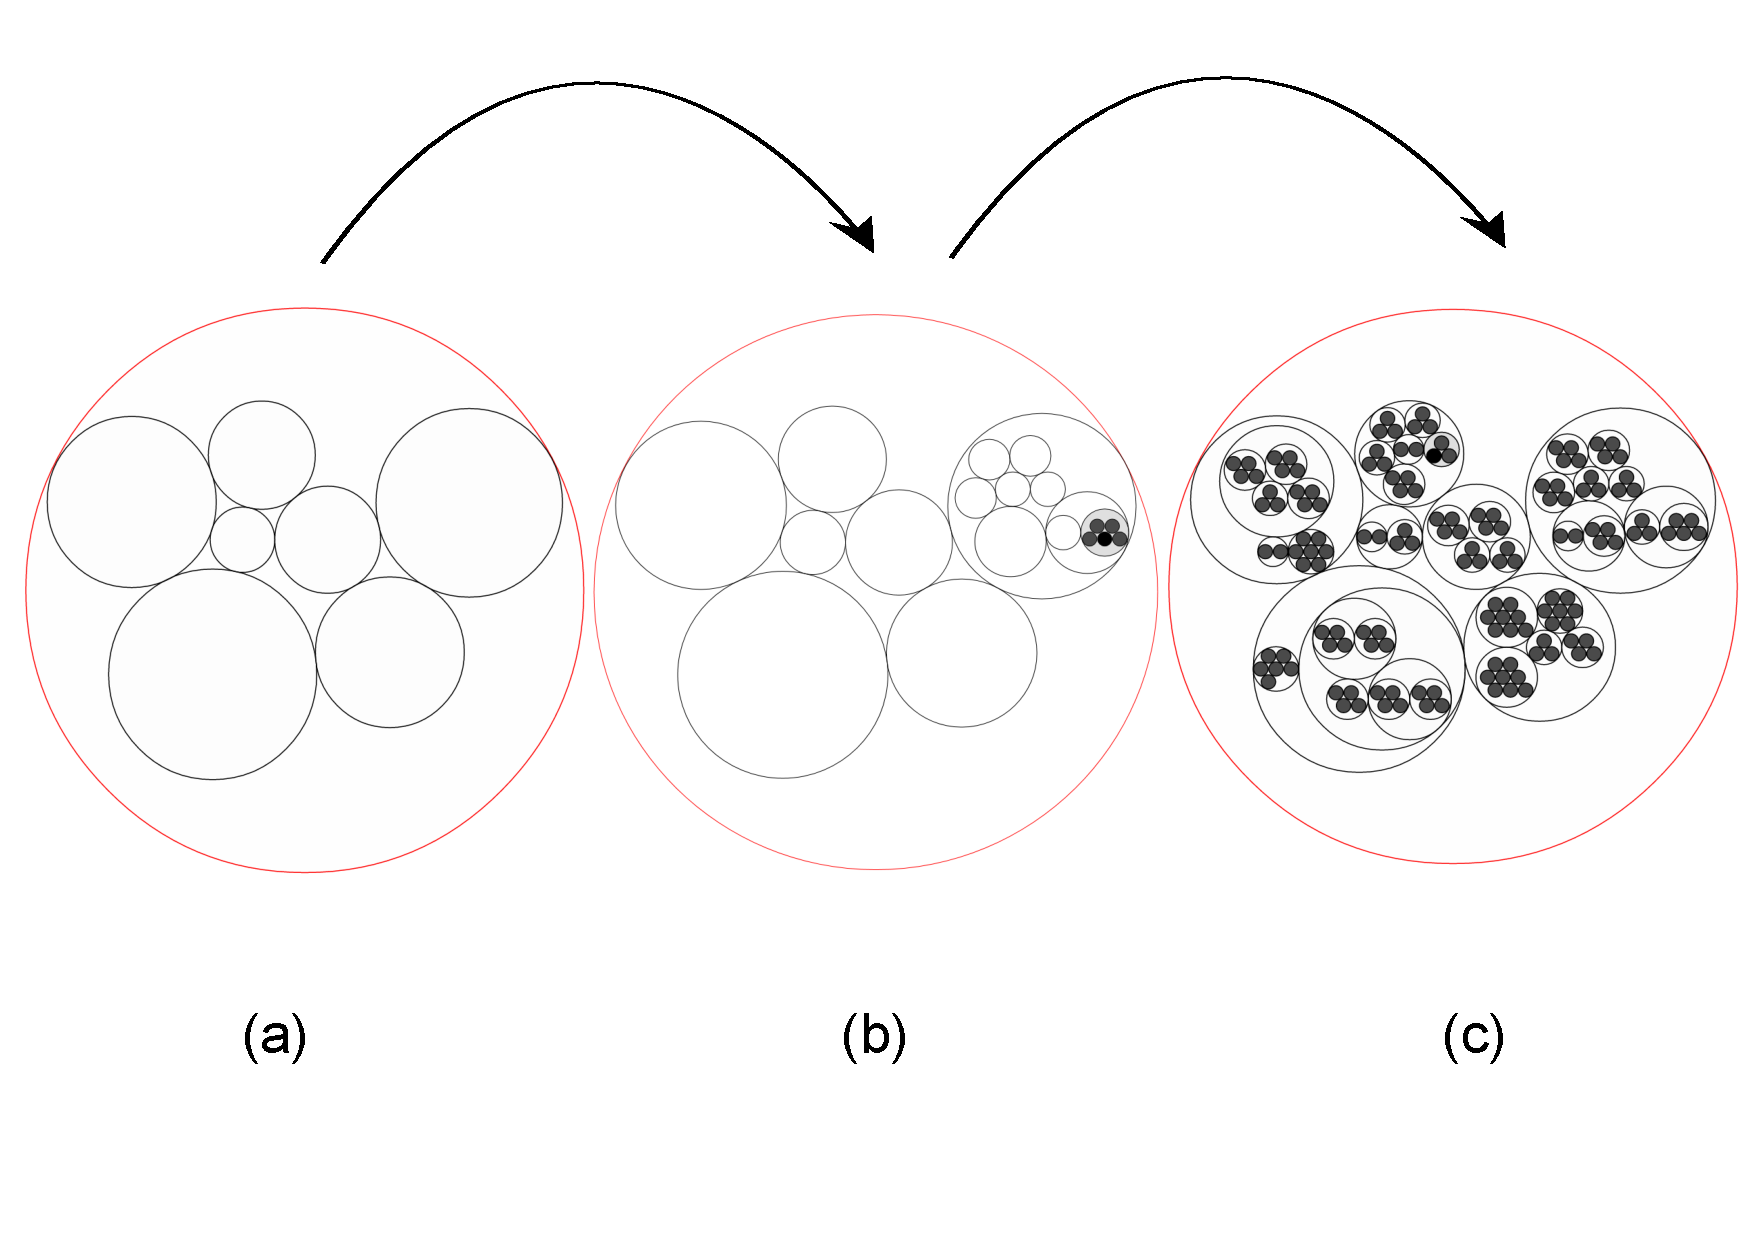
\includegraphics[scale=0.4]{gfx/XP1clean2.pdf} 
\end{center}
\caption{\label{figXP1} Progressive Semantic Display (PSD):  explicit hierarchical organization of semantic classes. (a) initial folded version; (b) partly folded version; (c) unfolded version}
\end{figure*}



The aim of the displays presented in this section is to allow the user to efficiently browse the above presented dataset of sounds explore without any written textual help. For each display, a sound is graphically represented by a filled circle whose, once clicked, plays the actual sound. The spatial organization is specific to each display.

As a reference, an Acoustic Display (AD) provides a spatial representation based on acoustic descriptors. For describing each sound, mel-frequency cepstrum coefficients (MFCCs) are computed with standard parameter settings (13 lowest quefrency coefficients are kept out of 40). The Euclidean distance between time averaged features is then computed between each sounds. A non metric multidimensional scaling with Kruskal's normalized stress is then considered to project the data into two dimensions \ref{figXP3} according to this distance.

Two semantically oriented displays are then proposed, called respectively Semantic Display (FSD) and Progressive Semantic Display (PSD), respecively shown on Figures~\ref{figXP2} and \ref{figXP1}. Both display  consider the hierarchical structure of the dataset to organize sounds. Each sound class is represented by a filled circle. Circles are then packed together according to the hierarchical semantic organization of the dataset, as shown on Figure \ref{figSSF}. Thus, subclasses belonging to the same class are close to each others. Circle packing functions of the D3.js (Data-Driven Documents) javascript library \cite{2011-d3} are used to distribute the sound classes in the space. Depending on the display, the user can whether acces directly to each leaf class or has to go through intermediate levels of the hierarchy. More precisely: \\
\begin{itemize}
\item \textit{FSD}: users can directly visualize the whole hierarchy, down to the leaf classes. Those leaf classes are distributed  in the same manner as PD. In that sense, the spatial configuration of the unfolded version of PD, which may be obtained after discovering all the classes and subclasses, is similar to that of  FD, as shown on Figures~\ref{figXP2}, \ref{figXP1} and \ref{figSSF}.
\item \textit{PSD}: users have access to the intermediate semantic levels of the hierarchy. Upon first using PD, they observe circles representing the top classes of the semantic hierarchical structure of the dataset. When users click on a circle, they hear the sound prototype of the class and the subclasses are progressively revealed, represented by white circles contained in the circle that has just been clicked. The same action repeats itself until the user reaches the leaf classes of the hierarchy. The leaf classes are represented with small gray circles, indicating that there is no subclass to discover. Thus the PD has a constrained exploration system. When a user click on a circle, sub-circles are  automatically revealed to him in a gradual way. Each time a sub-circle is automatically revealed, its sound prototype is played. Users may stop the discovery process by clicking on an other circle. 
\end{itemize}

The two interfaces have been designed in order to see whether a progressive top-down display of the hierarchical structure helps the user explore the dataset.

\section{Experiment} \label{test}

\subsection{Objective}

During this experiment, the three displays are compared. By comparing AD and xSD (the two semantic displays), the goal is to evaluate the  relative efficiencies of semantic based and acoustic based spatial configurations. By comparing FSD and PSD, we study the impact of an enforced hierarchical exploration of the corpus by the user. The goal is to check if constraining the user to browse the high levels of the hierarchy helps him to grasp and memorize the spatial configuration and the organization of the sound classes. 

\subsection{Experimental protocol}

We evaluate and compare those three displays with a crowdsourcing web-based experiment \footnote{The test is available at \url{http://217.70.189.118/soundthings/speedSoundFinding}} for which we adopt a between subject approach, \textit{i.e.} a subject can only test one display. In this experiment, subjects are asked to successively retrieve 13 target sounds among the 149 of the whole dataset. The target sounds are selected such as there are at least two target sounds in each top-level class of the semantic hierarchical structure of the dataset. To reduce order effects, target sounds are randomly presented to each subject.

First, the subject click a \textit{Play target sound} button to listen to the target sound. Then, the subject may replay the target sound  as many times as he likes. A timer starts when the subject clicks on a circle for the first time. When the target sound is found, subject puts an end to its search by clicking on the \textit{Click if found} button. This action 1) stops the timer and 2) loads a new target sound. If the subject does not find the correct target sound, an error message appears, and the experiment goes on with the same target sound.

During the experiment, two visual cues are shown to the subject:
\begin{itemize}
\item \textit{The search state}: which can be "pause" if the subject is currently not looking for a target sound (at the beginning of the experiment, or between two target sounds) or  "in progress"  if the subject is currently looking for a target sound.
\item \textit{Remaining target sounds}: the number of target sounds which remain to find.
\end{itemize}

The experiment ends when all the target sounds have been found. One shall notice that the PSD display is not reintialized at each change of the target sound. Thus, when a circle is unfolded, it remains visible during the whole experiment.

\subsection{Data Collection}
Four types of data are collected during the experiment:
\begin{itemize}
\item the total duration of the entire experiment. It includes breaks between two target sound searches and it is called the \textit{absolute duration}.
\item the duration of each search. The sum of the 13 search durations, which is the \textit{absolute duration} minus the break times between two target sound searches, is called the \textit{total search duration}.
\item the name of each sound which has been heard.
\item the time at which each sound has been heard.  
\end{itemize}

\subsection{Apparatus}

A crowdsourcing approach is adopted. The experiment is designed to be performed using the  \textit{chrome} web browser. The link to the experiment has been sent to three  mailing lists, namely \textit{Music-Ir, Auditory} and an internal IRCAM mailing list. Subjects are only allowed to perform the experiment once, and on one interface only. Data were automatically collected server-side at the end of the experiment. Subjects were asked to use headphones. All sounds of the dataset are normalized to the same root mean square (RMS) level.

\subsection{Participants}

60 subjects have completed the experiment, 20 for each interface.

\subsection{Statistical analysis}

We use one-way ANOVA and two samples \textit{t} tests at the 5\% significance level to test for statistical significance. All statistical analysis are performed using native functions of the computing environment MATLAB.


\section{Results} \label{results}
\subsection{Outlier detection}

\begin{table}[t]
\caption{\label{tab1} Criterion used to detect outliers}
\begin{center}
\begin{tabular}{ccccc}
criterion      &  1  &  2  &  3  &  4  \\
\hline
outlier 1 (PD) & --- & --- & --- &  x  \\
outlier 2 (PD) &  x  & --- & --- & --- \\  
outlier 3 (AD) & --- & --- & --- &  x \\
outlier 4 (AD) &  x  &  x  &  x  & --- \\
outlier 5 (AD) &  x  & --- & --- & --- \\
\hline
\end{tabular}
\end{center}
\end{table} 

Outlier detection is an important step of any crowdsourcing experiment as experimenters do not control the environment in which the subjects perform the experiment \cite{komarov2013crowdsourcing,buchholz2011crowdsourcing}. A commonly used method to detect outliers in  human-computer interaction studies is to consider as outlier an observation  which deviates of at least $\pm2$ standard deviation ($STD$) from the average \cite{komarov2013crowdsourcing}. though, as this latter method is not robust to the presence of isolated extreme observations (as it is often the case for crowdsourcing experiment), we follow the  method proposed by proposed by \cite{komarov2013crowdsourcing} and used the inter-quartile range ($IQR$). With this approach, an observation is considered to be an outlier if its value is more than $3*IQR$ higher than the third quartile or more than $3*IQR$ lesser than the first quartile. This methods is applied in this study to the four following criteria :

\begin{enumerate}
\item the \textit{absolute duration}: to detect subjects who took abnormally long breaks between searches.
\item the \textit{total search duration}: to detect subjects who spent an abnormally long time to complete the experiment.
\item number of heard sounds: to detect subjects who had to hear an abnormally high number of sounds to complete the experiment.
\item the maximum number of times a target sound had to be heard before being found: to detect subjects who had difficulty to recognize the target sounds.
\end{enumerate}

Using the $IQR$ method, 5 subjects are detected as outliers and removed from the analysis. 2 subjects used PD and 3 subjects AD. The tables~\ref{tab1} show the criteria used to detect the 5 outliers. 3 subjects are detected by observing the \textit{absolute duration}. They spent respectively 50 minutes, 5 hours and 17.5 hours to complete the experiment. 1 subject is detected by observing the total search duration (46 minutes), and an other by observing the total number of heard sounds (1800 heard sounds, roughly 12 times the total size of the corpus). And lastly 2 subjects are detected by observing the maximum number of times they had to hear a target sounds before finding it (4 and 8 times).

\begin{figure}[t]
\begin{center}
\includegraphics[scale=0.4]{gfx/analyse1.eps} 
\end{center}
\caption{\label{fig1} Average and standard deviation for (a) the total search durations, (b) the number of heard sounds and (c) the number of unique heard sounds}
\end{figure}  

\begin{figure}[t]
\begin{center}
\includegraphics[scale=0.4]{gfx/analyse2.eps} 
\end{center}
\caption{\label{fig2} evolution of (a) the average search durations, (b) the average numbers of heard sounds, and (c) average the numbers of unique heard sounds at each target sound search. Lines are linear regression.}
\end{figure}


\subsection{Efficiency}

To characterize the relative efficiency of the three displays, three metrics are considered: 

\begin{itemize}
\item the \textit{total search duration}
\item the number of sounds heard \mathias{on met heard avant ou apres sounds ?} 
\item the number of unique sounds heard. By "unique" we mean that, if a same sound is heard 10 times during the 13 searches of the  experiment, it counts only for one. 
\end{itemize}

The first two metrics quantify the notion of efficiency by considering the time and the number of clicks needed to achieve the task, \textit{ie.} reach the target. The goal for those values is to be as low as possible. The third data allows us to measure the selectivity of the interfaces. A low number of unique heard sounds indicates that subjects understood the spatial organisation of the dataset, and use this knowledge to improve their searches. In contrary, a high number of heard sounds without duplication suggest that the subject did not understood the way circles are organized in space, and tends to play all the sounds at each search. The maximum number of unique heard sounds is the corpus size: 149 sounds.

The averages and standard deviations for the three metrics are presented on Figure \ref{fig1}. The type of display have a significant effect on the the \textit{total search duration} ($F[2,52]=3.63; p=0.03$), the number of heard sounds ($F[2,52]=5.65; p<0.01$) and the number of unique heard sounds ($F[2,52]=8.65; p<0.01$). Post hoc analysis on the total search time (Figure~\ref{fig1}~(a)) shows that FSD  perform better  than the other interfaces (FSD-PSD: $p=0.04$; FSD-AD: $p=0.02$), whereas PSD and AD seem to have similar results (PSD-AD: $p=0.88$).

Similar results are found for the numbers of heard sounds Figure~\ref{fig1}~(b). FSD significantly outperforms the other interfaces (FSD-PSD: $p=0.02$; FSD-ASD: $p<0.01$), whereas PSD and AD show similar outcomes (PSD-AD: $p=0.42$).

Figure~\ref{fig1}~(c) shows the results for the number of unique heard sounds. This time the results of AD are significantly lower than those of both PD and FD (AD-PD: $p<0.01$; AD-FD: $p<0.01$).  For AD, 75\% of the subjects heard more than 140 sounds, and 25\% heard at least 148 sounds, that is almost the entire database. Considering PSD, 75\% of subjects heard  less than 134 sounds, against 143 for FSD. This time PSD and FSD seem to perform equally (PD-FD: $p=0.58$)

According to those results, a hierarchical organization of the dataset based on semantic values (PSD and FSD) allows the users to retrieve the 13 target sounds 1) more efficiently, and 2) by listening to a smaller amount of sounds than an organization based on acoustic descriptors (AD). However, those two effects are significantly compromised when users have to parse the entire hierarchy to reach the first target sound, as in the PSD display. It seems that enforcing an explicit exploration of the hierarchy disturbs or confuses the user instead of allowing him to learn the semantically motivated spatial organization of the classes. 


\subsection{Learning phenomenon}

We now study if and how users  progressively acquire knowledge about the spatial organization of the classes. To do that, the evolution of the above described metrics with respect to the search indexes is considered. Three sets of collected data are used:

\begin{itemize}
\item the duration of each target sound search 
\item the number of heard sounds for each target sound search 
\item the number of unique heard sounds for each target sound search. 
\end{itemize}

Figure~\ref{fig2}~(a) shows the evolution of the average durations of each target sound search observed for AD, FSD and PSD. As shown by a linear regression of the data, there is an overall increase of efficiency with respect to the index of the search. For the duration and the number of heard sounds, the AD and PSD perform equivalently, whereas the FSD exhibit better performance. In the case of the number of unique heard sounds, the two semantic displays are equivalent. This latter result suggest that for both semantic displays, users have parsed the same range of the dataset. Although users of FSD have done so by listening to fewer sounds and more quickly. 

\section{Conclusion}

In this paper, two displays allowing users to explore a sound dataset without written textual help are presented. The interfaces distribute sounds represented by circles on a 2D space. The spatial organisation is driven by semantic features. The two graphical displays are assessed and compared to a third listening based interface in which spatial configuration depends upon acoustic features. The tests consist in data retrieval tasks. 
The Full-Display (FD), that allows users to directly visualize the leaf classes of the semantic hierarchical structure, proves to be the most effective interface for the task.

Two main conclusions may be derived from this experiment. First, a spatial configuration based on semantic features is more effective to retrieve target sounds than a spatial configuration based on acoustic features. Second, an imposed visualisation of the semantic hierarchical structure of the dataset does not help user to understand and learn the spatial configuration of the semantic class, but instead disturbs the navigation. 

In the dataset considered in this study, there are as many leaf classes as sounds in the dataset, which would be unrealistic for large datasets. Though the organization can easily be adapted by considering the leaf classes as \textit{collections} of semantically similar sound samples. Thus, two sounds of \textit{male-yelling} would be grouped into a  single leaf class with the tag \textit{male-yelling}. The leaf class would then also have a \textit{prototype sound} being the most representative item of the different \textit{male-yelling} sounds belonging to the leaf class.

%It has to be noted that the test datasets are relatively small in terms of leaf sound classes. It may be interesting to test the FD on a larger dataset. 
%
%To conclude, if this study goal was to investigate the viability of an audio based data mining interface, other studies addressing comparison between FD and keyword based interfaces remain to be conducted. 


\section{Acknowledgements}

Research project partly funded by ANR-11-JS03-005-01.

\bibliographystyle{abbrv}
\bibliography{sigproc}  % sigproc.bib is the name of the Bibliography in this case

%In particular, much consideration has been given in order to avoid any semantic bias. Indeed any selection process based on keyword searching would have influenced the subject choices, and makes impossible or inadvisable to run any kind of identification tasks. 
%
%In a previous study \cite{ssf} we found  that the perceptively inspired structured of the sound data set (on which depends the spatial configuration of the circles) offers a easy-to-navigate format that allows subject to quickly understand the spatial localization of the different sound element classes and thus  enable them to quickly find a sound after a short amount of time. 
%
%%The interface selection has been tested in a previous \textit{crowd-sourcing} experiment on 60 subject. The goal was to find 10 target sound. Results showed that this interface allows subject to learn the sound spatial organisation, and to quickly retrieve a sound after some trials. 
\end{document}
